\documentclass[tikz,border=10pt]{standalone}
\usepackage{tikz}
\usepackage{amsmath}
\usepackage{amssymb}
\usetikzlibrary{arrows.meta,decorations.markings,calc}

\begin{document}
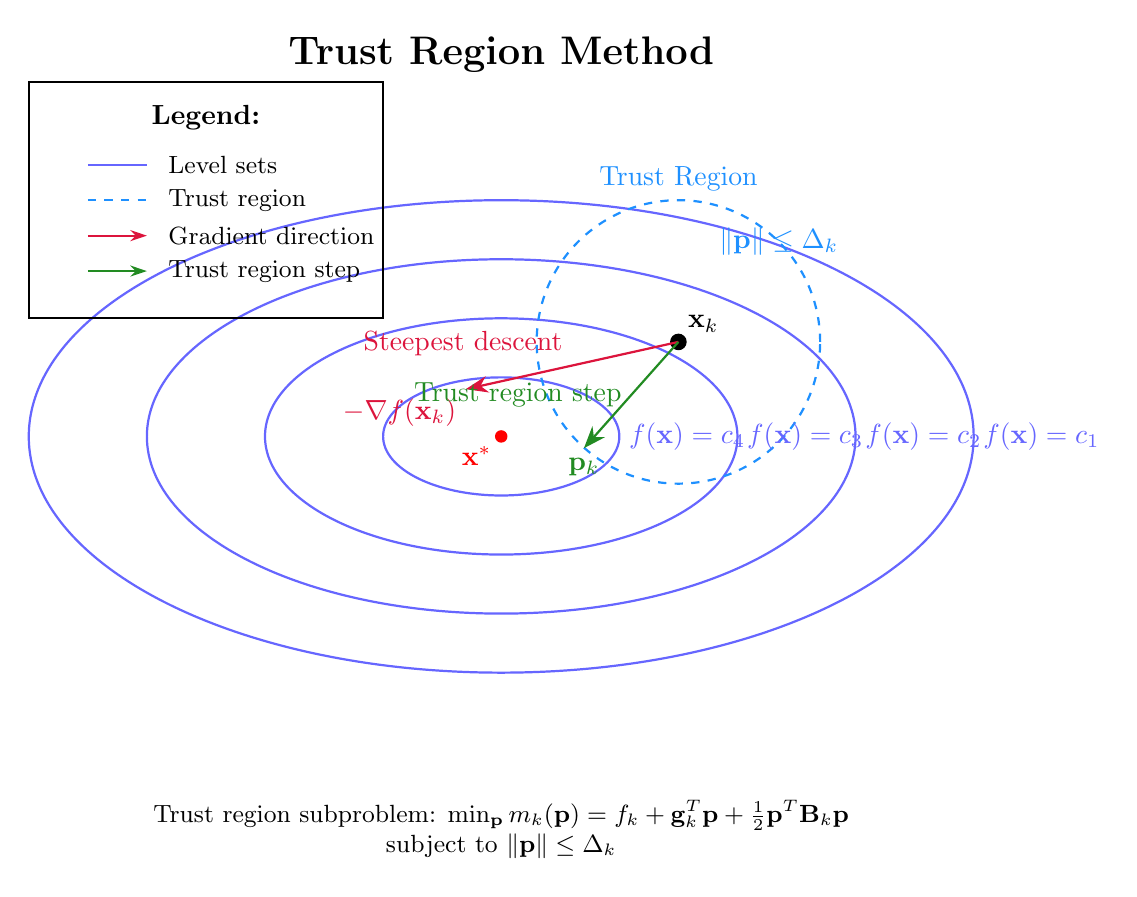
\begin{tikzpicture}[scale=1.5]
    % Define colors
    \definecolor{trustblue}{RGB}{30,144,255}
    \definecolor{gradred}{RGB}{220,20,60}
    \definecolor{stepgreen}{RGB}{34,139,34}
    
    % Draw level sets (contour lines)
    \draw[thick, blue!60] (0,0) ellipse (4 and 2);
    \draw[thick, blue!60] (0,0) ellipse (3 and 1.5);
    \draw[thick, blue!60] (0,0) ellipse (2 and 1);
    \draw[thick, blue!60] (0,0) ellipse (1 and 0.5);
    
    % Current point x_k
    \coordinate (xk) at (1.5, 0.8);
    \fill[black] (xk) circle (2pt);
    \node[above right] at (xk) {$\mathbf{x}_k$};
    
    % Trust region (circle)
    \draw[thick, trustblue, dashed] (xk) circle (1.2);
    \node[trustblue, above] at ($(xk) + (0, 1.2)$) {Trust Region};
    \node[trustblue] at ($(xk) + (0.85, 0.85)$) {$\|\mathbf{p}\| \leq \Delta_k$};
    
    % Steepest descent direction (negative gradient)
    \coordinate (grad_end) at ($(xk) + (-1.8, -0.4)$);
    \draw[-{Stealth[length=8pt,width=6pt]}, thick, gradred] 
        (xk) -- (grad_end);
    \node[gradred, below left] at (grad_end) {$-\nabla f(\mathbf{x}_k)$};
    \node[gradred, above left] at ($(xk) + (-0.9, -0.2)$) {Steepest descent};
    
    % Trust region step direction
    \coordinate (trust_step) at ($(xk) + (-0.8, -0.9)$);
    \draw[-{Stealth[length=8pt,width=6pt]}, thick, stepgreen] 
        (xk) -- (trust_step);
    \node[stepgreen, below] at (trust_step) {$\mathbf{p}_k$};
    \node[stepgreen, left] at ($(xk) + (-0.4, -0.45)$) {Trust region step};
    
    % Optimum point (center of ellipses)
    \fill[red] (0,0) circle (1.5pt);
    \node[red, below left] at (0,0) {$\mathbf{x}^*$};
    
    % Add labels for level sets
    \node[blue!60, right] at (4, 0) {$f(\mathbf{x}) = c_1$};
    \node[blue!60, right] at (3, 0) {$f(\mathbf{x}) = c_2$};
    \node[blue!60, right] at (2, 0) {$f(\mathbf{x}) = c_3$};
    \node[blue!60, right] at (1, 0) {$f(\mathbf{x}) = c_4$};
    
    % Add title
    \node[above, font=\Large\bfseries] at (0, 3) {Trust Region Method};
    
    % Add a small legend box
    \begin{scope}[shift={(-3.5, 2)}]
        \draw[thick] (-0.5, -1) rectangle (2.5, 1);
        \node[font=\bfseries] at (1, 0.7) {Legend:};
        \draw[thick, blue!60] (0, 0.3) -- (0.5, 0.3);
        \node[right, font=\small] at (0.6, 0.3) {Level sets};
        \draw[thick, trustblue, dashed] (0, 0) -- (0.5, 0);
        \node[right, font=\small] at (0.6, 0) {Trust region};
        \draw[-{Stealth[length=6pt,width=4pt]}, thick, gradred] (0, -0.3) -- (0.5, -0.3);
        \node[right, font=\small] at (0.6, -0.3) {Gradient direction};
        \draw[-{Stealth[length=6pt,width=4pt]}, thick, stepgreen] (0, -0.6) -- (0.5, -0.6);
        \node[right, font=\small] at (0.6, -0.6) {Trust region step};
    \end{scope}
    
    % Add mathematical description
    \node[below, align=center, font=\small] at (0, -3) {
        Trust region subproblem: $\min_{\mathbf{p}} m_k(\mathbf{p}) = f_k + \mathbf{g}_k^T\mathbf{p} + \frac{1}{2}\mathbf{p}^T\mathbf{B}_k\mathbf{p}$ \\
        subject to $\|\mathbf{p}\| \leq \Delta_k$
    };
    
\end{tikzpicture}
\end{document}
